\begin{problem}
Find an example of a finitely generated ring extension $R\subset
S$ where $S$ is a Noetherian ring, but $R$ is not.
\end{problem}
\begin{proof}
Let $k$ be a field and consider its polynomial ring $k[X,Y]$ in
two variables. Then we claim that the subring
$k[XY,XY^2,...]$ is non-Noetherian but its extension to
$k[X,Y]$ (by adjoining the indeterminants $X$ and $Y$)
is Noetherian by Hilbert's basis theorem. Consider the increasing
chain of ideals
\[
(XY)\subsetneq (XY,XY^2)\subsetneq(XY,XY^2,XY^3)\subsetneq\cdots.
\]
This chain does not stabilize for suppose that it did, then for
some positive integer $n$, we have
$(XY,XY^2,...,XY^n)=(XY,XY^2,...,XY^n,XY^{n+1})$ so
$XY^{n+1}\in(XY,XY^2,...,XY^n)$. But this implies that
$XY^{n+1}=p(XY,XY^2,...)q(XY,...,XY^n)$ for some polynomials $q\in
k[XY,XY^2,...]$, $q\in(XY,...,XY^n)$. Thus, we have that
\begin{align*}
\deg_Y(XY^{n+1})
&=n+1
&\deg_X(XY^{n+1})
&=1
\\
&=\deg_Y p+\deg_Y q
&&=\deg_X p+\deg_X q.
\end{align*}
Since $\deg_Y q\leq n$, $\deg_Y p\geq 1$. Thus, $\deg_X p=1$ so
$q\in k$, i.e., $q$ is a unit. This is a contradiction since
$(XY,...,XY^n)$ is a proper ideal.
\end{proof}
\newpage
\begin{problem}
Consider the homomorphism of rings
\begin{center}
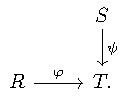
\includegraphics{figures/hw-4-ring-maps}
\end{center}
The \emph{fiber product} of $R$ and $S$ over $T$ is the subring
$R\times_T S=\left\{\,(r,s)\;\middle|\;\phi(t)=\psi(s)\,\right\}$
of $R\times S$. Assume $\phi$ and $\psi$ are surjective. Show
that if $R$ and $S$ are Noetherian rings then so is $R\times_T
S$.
\end{problem}
\begin{proof}
We first prove the following result:
\begin{lemma}[Matsumura, Ex.\,3.1]
Let $\mathfrak{a}_1,...,\mathfrak{a}_n$ be ideals of a ring $A$
such that $\mathfrak{a}_1\cap\cdots\cap\mathfrak{a}_n=0$. If each
$A/\mathfrak{a}_i$ is a Noetherian ring then so is $R$.
\end{lemma}
\begin{proof}[Proof of lemma]
\renewcommand\qedsymbol{$\clubsuit$}
If the $\mathfrak{a}_1,..,\mathfrak{a}_n$ are coprime, by
the Chinese remainder theorem, we have $A\cong
A_1/\mathfrak{a}_1\times\cdots A_n/\mathfrak{a}_n$ so $A$ is
Noetherian. Otherwise, we have a canonical injection
$\phi\colon A\hookrightarrow A_1/\mathfrak{a}_1\times\cdots\times
A_n/\mathfrak{a}_n$ which gives rise to the exact sequence of
$A$-modules
\begin{center}
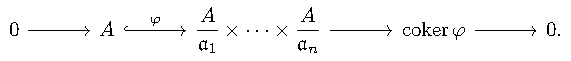
\includegraphics{figures/ps4-p2-short-exact-seq}
\end{center}
By 3.4(a), $R$ is Noetherian.
\end{proof}
Now consider the canonical projections $\pi_R\colon R\times_T
S\to R$ and $\pi_S\colon R\times_T S\to S$. Then, by the
isomorphism theorem we have $R\cong R\times_T S/\ker\pi_R$ and
$S\cong R\times_T S/\ker\pi_S$. Then we have the following
\begin{center}
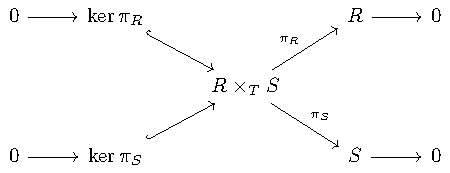
\includegraphics{figures/ps4-p2-short-exact-seqs}
\end{center}
which is short exact along the top and bottom, left to
right. Since
\[
R\times S\cong \frac{R\times_T S}{\ker\pi_R}\times\frac{R\times_T S}{\ker\pi_S}
\]
by Lemma 1, we need only show that
$\ker\pi_R\cap\ker\pi_S=0$. But this is straightforward for
suppose $(x,y)\in\ker\pi_R\cap\ker\pi_S$ then $(x,y)\in\ker\pi_R$
implies that $(x,y)=(0,y)$ for all $y\in\ker\psi$ and
$(x,y)\in\ker\pi_S$ implies that $(x,y)=(x,0)$ where
$x\in\ker\phi$ so $(x,y)=(0,0)$. Applying Lemma 1, it follows
that $R\times_T S$ is Noetherian.
\end{proof}
\newpage
\begin{problem}
Let $M$ be an $R$-module. Show that $M$ is a flat $R$-module if
and only if $M_{\mathfrak{m}}$ is a flat
$R_{\mathfrak{m}}$-module for every maximal ideal $\mathfrak{m}$
of $R$.
\end{problem}
\begin{proof}
We prove the following result:
\begin{lemma}[Atiyah \& MacDonald, Ex.2.8(i)]
If $M$ and $N$ are flat $A$-modules, then so is $M\otimes_A N$.
\end{lemma}
\begin{proof}[Proof of lemma]
\renewcommand\qedsymbol{$\clubsuit$}
Let
\[
0\longrightarrow
N'\longrightarrow
N\longrightarrow
N''\longrightarrow
0
\]
be a short exact sequence of $A$-modules. Since $M$ is a flat
$A$-module, by , the following is a short exact sequence
\[
0\longrightarrow
M\otimes N'\longrightarrow
M\otimes N\longrightarrow
M\otimes N''\longrightarrow
0.
\]
Moreover, since $N$ is also a flat $A$-module, the following is also short
exact
\[
0\longrightarrow
N\otimes(M\otimes N')\longrightarrow
N\otimes(M\otimes N)\longrightarrow
N\otimes(M\otimes N'')\longrightarrow
0
\]
so, by 2.7, we have that
\[
0\longrightarrow
(N\otimes M)\otimes N'\longrightarrow
(N\otimes M)\otimes N\longrightarrow
(N\otimes M)\otimes N''\longrightarrow
0
\]
is short exact. Hence, $N\otimes M$ is a flat $A$-module.
\end{proof}
Let $\mathfrak{m}\subset R$ be a maximal ideal. Then
$R_{\mathfrak{m}}$ is $R$-algebra via the canonical inclusion map
$\iota\colon R\hookrightarrow R_{\mathfrak{m}}$. Thus, $M$ admits
an $(R,R_{\mathfrak{p}})$-bimodule structure, by 2.8, so that given
an $R$-module $N$ and an $R_{\mathfrak{p}}$-module $P$ there is a
canonical isomorphism
\[
N\otimes_R (M\otimes_{R_{\mathfrak{m}}} P)\cong (N\otimes _R
M)\otimes_{R_{\mathfrak{m}}} P.
\]

Now, suppose that $M$ is a flat $R$-module. Then, given an
injective $R$-linear map $\phi\colon N\hookrightarrow P$ the
induced $R$-linear map
\[
M\otimes_R N
\hooklongrightarrow
M\otimes_R P
\]
is injective (in this case, the mapping is
$(m,n)\mapsto(m,\phi(n))$. But by 4.5 $(M\otimes_R
N)_{\mathfrak{m}}\cong (R_{\mathfrak{m}}\otimes_R
M)\otimes_{R_{\mathfrak{m}}}(R_{\mathfrak{m}}\otimes_R N)$ so by
4.6 and Lemma 2, the induced $R_{\mathfrak{m}}$-linear map
\[
M_{\mathfrak{m}}\otimes_{R_{\mathfrak{m}}} N_{\mathfrak{m}}\hooklongrightarrow
M_{\mathfrak{m}}\otimes_{R_{\mathfrak{m}}} N_{\mathfrak{m}}
\]
is injective (in this case, the mapping factors through a number
of isomorphism, but element-wise rule is not important). Hence,
$M_{\mathfrak{m}}$ is flat.

Conversely, suppose that $M_{\mathfrak{m}}$ is flat for every
maximal ideal $\mathfrak{m}\subset R$. Then, given an
injective $R_{\mathfrak{m}}$-linear map $\phi\colon
N\hookrightarrow P$ the induced map
\[
M_{\mathfrak{m}}\otimes_{R_{\mathfrak{m}}} N\hooklongrightarrow
M_{\mathfrak{m}}\otimes_{R_{\mathfrak{m}}} P
\]
is injective. By restriction of scalars, we make $N$ and $P$ into
$R$-modules via $N'=R_{\mathfrak{m}}\otimes_R N$ and
$M'=R_{\mathfrak{m}}\otimes_R P$ so $(M\otimes_R
N')_{\mathfrak{m}}\cong M_{\mathfrak{m}}\otimes_{R_{\mathfrak{m}}} N$ and $(M\otimes_R
P')_{\mathfrak{m}}\cong
M_{\mathfrak{m}}\otimes_{R_{\mathfrak{m}}} P$ so we have that the map
\[
(M\otimes_R N')_{\mathfrak{m}}\hooklongrightarrow (M\otimes_R P')_{\mathfrak{m}}
\]
is injective for all $\mathfrak{m}$. We claim that this implies
that the mapping
\[
\Phi\colon M\otimes_R N'\longrightarrow M\otimes_R P'
\]
is injective. Consider the short exact sequence
\[
0\longrightarrow
\ker\Phi\longrightarrow
M\otimes_R N'\longrightarrow
M\otimes_R P'\longrightarrow
0.
\]
By assumption, when we localize we have an injection $(M\otimes_R
N')_{\mathfrak{m}}\hookrightarrow (M\otimes_R P')_{\mathfrak{m}}$ so
\[
0\longrightarrow
(\ker\Phi)_{\mathfrak{m}}\longrightarrow
(M\otimes_R N')_{\mathfrak{m}}\hooklongrightarrow
(M\otimes_R P')_{\mathfrak{m}}\longrightarrow
0
\]
implies that $(\ker\Phi)_{\mathfrak{m}}=0$ for all
$\mathfrak{m}$. By 4.9, this implies that $\ker\Phi=0$ so the map
$\Phi$ is indeed an injection. Thus, $M$ is a flat $R$-module.
\end{proof}
\newpage
\begin{problem}
Let $M$ be an $R$-module and $\mathfrak{a}$ an $R$-ideal.
\begin{enumerate}[noitemsep,label=(\alph*)]
\item Show that if $M_{\mathfrak{m}}=0$ for every maximal ideal
  $\mathfrak{m}$ containing $\mathfrak{a}$, then $M=\mathfrak{a}M$.
\item Show that the converse holds in case $M$ is finite.
\end{enumerate}
\end{problem}
\begin{proof}
(a) Consider the quotient ring $R/\mathfrak{a}$. The pair
$(R/\mathfrak{a},\pi)$, where $\pi\colon R\twoheadrightarrow
R/\mathfrak{a}$ is the canonical projection, is an $R$-algebra so
it makes sense to talk about restriction of scalars. Now, by
2.13, we have that $R/\mathfrak{a}\otimes_R M\cong
M/\mathfrak{a}M$ is an $R/\mathfrak{a}$-module. By 1.2, there is
a one-one correspondence between maximal ideals
$\overbar{\mathfrak{m}}$ of $R/\mathfrak{a}$ and maximal ideals
$\mathfrak{m}\supset\mathfrak{a}$. Thus,
$(M/\mathfrak{a}M)_{\overbar{\mathfrak{m}}}=0$ for every maximal ideal
$\overbar{\mathfrak{m}}$ implies, by 4.9, that $(M/\mathfrak{a}M)=0$. Thus,
$M=\mathfrak{a}M$.
\\\\
(b) Now suppose $M$ is finitely generated and
$M=\mathfrak{a}M$. Then, by Nakayama's lemma, there exists $x\in
1+\mathfrak{a}$ such that $xM=0$. In particular, we have that
$x\in\ann M$ so by 4.8, $x/1\in\ann_{R_{\mathfrak{m}}}
M_\mathfrak{m}$. However, $x/1$ is a unit in $M_{\mathfrak{m}}$
(since $x\notin\mathfrak{m}$) so $(x/1)M_{\mathfrak{m}}=0$, but
$(x/1)M_{\mathfrak{m}}=M_{\mathfrak{m}}$ so
$M_{\mathfrak{m}}=0$.
\end{proof}
\newpage
\begin{problem}
Prove that every power of a maximal ideal is primary.
\end{problem}
\begin{proof}
Let $R$ be a ring, $\mathfrak{m}\subset R$ be a maximal ideal and
$k$ a positive integer. Consider the quotient
$R/\mathfrak{m}^k$. We must show that every zero-divisor of
$R/\mathfrak{m}^k$ is nilpotent. Note that $R/\mathfrak{m}^k$ is
a local ring with maximal ideal $\overbar{\mathfrak{m}}$ the
projection of $\mathfrak{m}$ (for suppose
$\overbar{\mathfrak{n}}$ is another maximal ideal of
$R/\mathfrak{m}^k$, then, by 1.2, there is a corresponding
maximal ideal $\mathfrak{n}\supset\mathfrak{m}^k$ of $R$, but
$\sqrt{\mathfrak{m}^k}=\mathfrak{m}\subset\mathfrak{n}$ implies
$\mathfrak{m}=\mathfrak{n}$ by maximality). Suppose $\bar x\bar
y=\bar 0$ where $\bar x\neq\bar 0$ and $\bar y\neq \bar 0$ are in
$R/\mathfrak{m}^k$. Then, if either $\bar x$ or $\bar y$ is a
unit we are done. Suppose $\bar x$ and $\bar y$ are
non-units. Then $\bar x,\bar y\in\overbar{\mathfrak{m}}$ so $\bar
x^k=\bar y^k=\bar 0$ are nilpotent since
$x^k,y^k\in\mathfrak{m}^k$. It follows that $\mathfrak{m}^k$ is
primary.
\end{proof}
\newpage
\begin{problem}
\begin{enumerate}[noitemsep,label=(\alph*)]
\item Show that the radical of a primary ideal is prime.
\item Find an example of a power of a prime ideal that is not
  primary.
\item Let $\mathfrak{p}$ be a prime ideal of a ring $R$ and
  $n\in\NN$. The $R$-ideal
  $\mathfrak{p}^{(n)}=R\cap\mathfrak{p}^nR_{\mathfrak{p}}$ is
  called the \emph{$n$th symbolic power of $\mathfrak{p}$}. Show
  that $\mathfrak{p}^{(n)}$ is primary.
\end{enumerate}
\end{problem}
\begin{proof}
(a) Let $\mathfrak{a}\subset R$ be primary. Suppose
$xy\in\sqrt{\mathfrak{a}}$. Then $x^ky^k\in\mathfrak{a}$. Since
$\mathfrak{a}$ is primary, either $x^k\in\mathfrak{a}$ (in which
case, $x\in\mathfrak{a}$) or $y\in\sqrt{\mathfrak{a}}$. In either
case, $x\in\sqrt{\mathfrak{a}}$ or $y\in\sqrt{\mathfrak{a}}$
hence, $\sqrt{\mathfrak{a}}$ is prime.
\\\\
(b) Consider the following example (taken from Atiyah \& MacDonald
\S4, Example 2): Consider the quotient of the polynomial ring in
three variables $A=k[X,Y,Z]/(XY-Z^2)$ and let $\overbar{X}$,
$\overbar{Y}$ and $\overbar{Z}$ be the images of $X$, $Y$ and
$Z$, respectively, in the quotient. Then
$\mathfrak{p}=(\overbar{X},\overbar{Z})$ is prime (since
$A/\mathfrak{p}\cong k[Y]$ via
$\overbar{Y}+\mathfrak{p}\mapsto Y$ is a domain)
however $\mathfrak{p}^2$ is not primary since
\[
\overbar{X}\overbar{Y}=XY+(XY-Z^2)=Z^2+(XY-Z^2)=\overbar{Z}^2\in\mathfrak{p}^2,
\]
but $\overbar{X}\notin\mathfrak{p}^2$ and
$\overbar{Y}\notin\sqrt{\mathfrak{p}^2}=\mathfrak{p}$. Hence,
$\mathfrak{p}^2$ is not primary.
\\\\
(c) Note that that since $\mathfrak{p}^n\subset\mathfrak{p}$ then
$(\mathfrak{p}^n)^e\subset\mathfrak{p}^e$ so by 4.13(c)
$(\mathfrak{p}^n)^{ec}\subset\mathfrak{p}^{ec}=\mathfrak{p}$ so
by 4.13(e) it suffices to show that $(\mathfrak{p}^n)^e$ is
primary. But this follows from Problem 3.5 since
$(\mathfrak{p}^n)^e$ is a power of the unique maximal ideal
$\mathfrak{p}R_{\mathfrak{p}}$ of the local ring
$R_{\mathfrak{p}}$.
\end{proof}

%%% Local Variables:
%%% mode: latex
%%% TeX-master: "../MA557-HW-Current"
%%% End:
